% Options for packages loaded elsewhere
\PassOptionsToPackage{unicode}{hyperref}
\PassOptionsToPackage{hyphens}{url}
\PassOptionsToPackage{dvipsnames,svgnames,x11names}{xcolor}
%
\documentclass[
  10pt,
  a4paper,
]{article}
\usepackage{amsmath,amssymb}
\usepackage{iftex}
\ifPDFTeX
  \usepackage[T1]{fontenc}
  \usepackage[utf8]{inputenc}
  \usepackage{textcomp} % provide euro and other symbols
\else % if luatex or xetex
  \usepackage{unicode-math} % this also loads fontspec
  \defaultfontfeatures{Scale=MatchLowercase}
  \defaultfontfeatures[\rmfamily]{Ligatures=TeX,Scale=1}
\fi
\usepackage{lmodern}
\ifPDFTeX\else
  % xetex/luatex font selection
\fi
% Use upquote if available, for straight quotes in verbatim environments
\IfFileExists{upquote.sty}{\usepackage{upquote}}{}
\IfFileExists{microtype.sty}{% use microtype if available
  \usepackage[]{microtype}
  \UseMicrotypeSet[protrusion]{basicmath} % disable protrusion for tt fonts
}{}
\makeatletter
\@ifundefined{KOMAClassName}{% if non-KOMA class
  \IfFileExists{parskip.sty}{%
    \usepackage{parskip}
  }{% else
    \setlength{\parindent}{0pt}
    \setlength{\parskip}{6pt plus 2pt minus 1pt}}
}{% if KOMA class
  \KOMAoptions{parskip=half}}
\makeatother
\usepackage{xcolor}
\usepackage[margin=21mm]{geometry}
\usepackage{longtable,booktabs,array}
\usepackage{calc} % for calculating minipage widths
% Correct order of tables after \paragraph or \subparagraph
\usepackage{etoolbox}
\makeatletter
\patchcmd\longtable{\par}{\if@noskipsec\mbox{}\fi\par}{}{}
\makeatother
% Allow footnotes in longtable head/foot
\IfFileExists{footnotehyper.sty}{\usepackage{footnotehyper}}{\usepackage{footnote}}
\makesavenoteenv{longtable}
\usepackage{graphicx}
\makeatletter
\def\maxwidth{\ifdim\Gin@nat@width>\linewidth\linewidth\else\Gin@nat@width\fi}
\def\maxheight{\ifdim\Gin@nat@height>\textheight\textheight\else\Gin@nat@height\fi}
\makeatother
% Scale images if necessary, so that they will not overflow the page
% margins by default, and it is still possible to overwrite the defaults
% using explicit options in \includegraphics[width, height, ...]{}
\setkeys{Gin}{width=\maxwidth,height=\maxheight,keepaspectratio}
% Set default figure placement to htbp
\makeatletter
\def\fps@figure{htbp}
\makeatother
\setlength{\emergencystretch}{3em} % prevent overfull lines
\providecommand{\tightlist}{%
  \setlength{\itemsep}{0pt}\setlength{\parskip}{0pt}}
\setcounter{secnumdepth}{-\maxdimen} % remove section numbering
\usepackage{amsmath,amssymb,mathtools}
\usepackage{fontspec}
\usepackage{unicode-math}
\setmainfont{Noto Serif}
\setsansfont{Noto Sans}
\setmonofont{DejaVu Sans Mono}[Scale=0.78]
\setmathfont{latinmodern-math.otf}
\usepackage{xurl}
\usepackage{fvextra}
\DefineVerbatimEnvironment{Highlighting}{Verbatim}{breaklines,commandchars=\\\{\}}
\usepackage{microtype}
\usepackage{fancyhdr}
\usepackage{etoolbox}
\usepackage{needspace}
\pagestyle{fancy}
\fancyhf{}
\fancyhead[L]{\footnotesize Research review edition}
\fancyhead[R]{\footnotesize 26 September 2026}
\fancyfoot[R]{\thepage}
\renewcommand{\headrulewidth}{0.3pt}
\setlength{\headheight}{14pt}
\setlength{\emergencystretch}{3em}
\setlength{\parskip}{5pt}
\setlength{\tabcolsep}{4pt}
\renewcommand{\arraystretch}{1.13}
\AtBeginEnvironment{longtable}{\footnotesize}
\AtBeginEnvironment{quote}{\small}
\allowdisplaybreaks
\makeatletter
\renewcommand\section{\@startsection{section}{1}{\z@}{-2.4ex \@plus -1ex \@minus -.2ex}{1.2ex \@plus .2ex}{\normalfont\Large\bfseries}}
\renewcommand\subsection{\@startsection{subsection}{2}{\z@}{-2ex \@plus -.8ex \@minus -.2ex}{.9ex \@plus .2ex}{\normalfont\large\bfseries}}
\makeatother
\ifLuaTeX
  \usepackage{selnolig}  % disable illegal ligatures
\fi
\usepackage{bookmark}
\IfFileExists{xurl.sty}{\usepackage{xurl}}{} % add URL line breaks if available
\urlstyle{same}
\hypersetup{
  colorlinks=true,
  linkcolor={Maroon},
  filecolor={Maroon},
  citecolor={Blue},
  urlcolor={black},
  pdfcreator={LaTeX via pandoc}}

\author{}
\date{}

\begin{document}

\section{Absolute Infinite Union}\label{absolute-infinite-union}

\subsection{A critical case for a generative
substrate}\label{a-critical-case-for-a-generative-substrate}

\textbf{James McGaughran}

MathGov / RippleLogic Research Program

26 September 2026 \textbar{} Review manuscript v1.4

\subsection{Abstract}\label{abstract}

Absolute Infinite Union is examined as the hypothesis that
differentiated existence depends on one unbounded generative reality,
potentially experiential and, in its strongest version, one subject with
genuine local perspectives. Totality, monist grounding, unboundedness,
lawful generation, realized possibilities, experiential fundamentality
and cosmic subjectivity are separate commitments. The paper combines an
affirmative philosophical case with an explicit map of the bridges
needed for scientific support. Its constructive result is conditional: a
stationary ergodic symbolic process realizes every supported finite word
infinitely often almost surely. The extension to nonergodic processes
shows why shared support across components, not ergodicity alone, is the
decisive issue for pattern coverage. These standard probabilistic tools
clarify premises but do not identify the physical universe or turn
descriptions into experiencing worlds. A finite-observation comparison
illustrates experiment-specific underdetermination. Primary-source
approaches to subject differentiation are examined alongside structural,
neutral-monist and physical-realization rivals; passage-level and
abstract-only checks remain distinguished. The distinction between
common grounding and phenomenal unity prevents arguments for monism from
silently becoming arguments for a cosmic subject. Neither repeated
oneness reports nor a correct quantum-record theorem determine an
ontological likelihood without an observation model. The conclusion is a
positive, corrigible research position, not a proof of AIU, its
negation, or a numerical probability of ultimate reality.

\subsection{1. The hypothesis we are actually
investigating}\label{the-hypothesis-we-are-actually-investigating}

The motivating picture is not simply that the universe is very large. It
is that all differentiated existence may be the activity or
configuration of one fundamental reality. This ground would not merely
occupy a pre-existing container. On a strong version, the forms we call
spacetime, matter, organisms and subjects are its expressions. The
further proposal is that the ground is unbounded, intrinsically
experiential and generative of every possibility. The image of one
consciousness dreaming many worlds expresses this stronger position.

This paper takes that target seriously. It does not quietly reduce AIU
to ordinary ecological interdependence, and it does not grant the target
as a premise of its own proof. The question is whether the conjunction
can be defined coherently, explained economically, connected to
observations and preferred over its strongest rivals.

A distinction in attitude is useful. A researcher can have a strong
personal expectation that a hypothesis will prove correct while making
public claims at the level the evidence currently supports. Such an
expectation can direct attention and sustain investigation. It cannot
determine the verdict of the tests. A research programme becomes weaker,
not stronger, when every adverse result is redescribed as another
manifestation of its preferred conclusion.

The best scientific interpretation of the author's determination is
therefore a commitment to expose AIU to meaningful challenge. The
project succeeds by learning which propositions survive, even if the
final account differs from the initiating image. It does not succeed
merely by finding more words for unity.

\subsubsection{Contribution and limits}\label{contribution-and-limits}

The paper's contribution is an integrated philosophical argument: a
seven-part decomposition of the strong hypothesis, explicit inference
bridges, a componentwise criterion for finite-pattern coverage, a
restricted finite-observation comparison, and a primary-source
comparison of subject accounts. The probability results apply
established tools; the taxonomy and their joint use are not asserted to
be historically unique. A worked pair of subject models below makes one
precise point of disagreement available for criticism without claiming a
new consciousness mechanism or a proof of the proposed ontology.

\subsection{2. Definitions that preserve the strong
thesis}\label{definitions-that-preserve-the-strong-thesis}

Table 1 separates propositions that otherwise move between meanings.
Here AIU means \textbf{Absolute Infinite Union}. Its content is fixed by
the explicit commitments below, not by the acronym or the metaphors
associated with it. A unity-of-reality definition must not silently
import an infinite ground, plenitude or one cosmic subject.

\Needspace{12\baselineskip}

\textbf{Table 1. The claims carried by the strongest AIU proposal}

\begin{longtable}[]{@{}
  >{\raggedright\arraybackslash}p{(\columnwidth - 4\tabcolsep) * \real{0.3333}}
  >{\raggedright\arraybackslash}p{(\columnwidth - 4\tabcolsep) * \real{0.3333}}
  >{\raggedright\arraybackslash}p{(\columnwidth - 4\tabcolsep) * \real{0.3333}}@{}}
\toprule\noalign{}
\begin{minipage}[b]{\linewidth}\raggedright
Claim
\end{minipage} & \begin{minipage}[b]{\linewidth}\raggedright
Precise working content
\end{minipage} & \begin{minipage}[b]{\linewidth}\raggedright
Kind and present status
\end{minipage} \\
\midrule\noalign{}
\endhead
\bottomrule\noalign{}
\endlastfoot
T: totality & Everything actual is included in what we call reality &
Definitional; does not establish one substance \\
M: one ground & No actual entity is ontologically independent of one
fundamental generative ground & Metaphysical hypothesis \\
U: unboundedness & A named property of that ground has no finite global
bound & Open physical or metaphysical claim, depending on the bearer \\
G: form generation & Differentiated effective structures are grounded in
or arise from that basis under specified relations & Model-dependent;
demonstrated in restricted systems, not universally \\
P: plenitude & Every possibility in a declared admissible class is
actually realized & Strong additional realization claim \\
C: experiential fundamentality & Experience is a fundamental aspect of
the generative ground & Metaphysical hypothesis \\
C*: cosmic subjectivity & One unified subject grounds genuine local
perspectives & Additional metaphysical hypothesis with individuation
obligations \\
\end{longtable}

The preferred strong thesis is not T alone. The author's strongest
version is \(M\land U\land P\land C\land C^{\text{*}}\), with a
generative account G. The conjunction's meaning depends on the
definitions of U, P and C. Infinite spatial volume, unlimited global
distinguishable capacity, all finite patterns, all physical histories
and all logically coherent worlds are different theses. So are a ground
with experiential aspects and a single phenomenally unified cosmic
subject.

For M, grounding need not mean temporal production. If time is itself
effective, asking what happened before the ground formed its first state
may import the wrong relation. A non-temporal dependence account must
nevertheless explain why particular effective structures exist. Calling
the relation grounding does not remove the need for a clear mechanism or
philosophical argument.

For U, an operational variant could say that, as the declared finite
domain and its resources are enlarged, no finite bound exists on the
number of globally available distinguishable alternatives at a fixed
error tolerance. This is stronger than the observation that a qubit has
continuously many pure states, but weaker than a largest mathematical
infinity. It does not imply that one observer can access the entire
domain. Other U variants must be stated separately rather than treated
as interchangeable confirmations.

For P, the minimal useful version concerns every finite configuration
allowed by a fixed law and realization measure. A maximal version
extends to every coherent reality under every law. The latter needs a
theory of coherence, equivalence and observation across that vast
domain. It is not licensed by a theorem about one infinite sequence.

For C*, the central task is subject individuation. Why are there private
viewpoints, limited memories and local access rather than one publicly
available total experience? An answer must preserve the reality of those
limits instead of defining them as illusions whenever they create a
difficulty.

\subsubsection{2.1 Commitments and evidence
bridges}\label{commitments-and-evidence-bridges}

Mathematical method, physical recovery and ontological interpretation
need not succeed or fail together. Table 2 distinguishes the immediate
conclusion of each type of result from the additional bridge required
for the next claim.

\Needspace{12\baselineskip}

\textbf{Table 2. What each result could license, and what remains to be
supplied}

\begin{longtable}[]{@{}
  >{\raggedright\arraybackslash}p{(\columnwidth - 4\tabcolsep) * \real{0.3333}}
  >{\raggedright\arraybackslash}p{(\columnwidth - 4\tabcolsep) * \real{0.3333}}
  >{\raggedright\arraybackslash}p{(\columnwidth - 4\tabcolsep) * \real{0.3333}}@{}}
\toprule\noalign{}
\begin{minipage}[b]{\linewidth}\raggedright
Starting point
\end{minipage} & \begin{minipage}[b]{\linewidth}\raggedright
Legitimate immediate conclusion
\end{minipage} & \begin{minipage}[b]{\linewidth}\raggedright
Further bridge required
\end{minipage} \\
\midrule\noalign{}
\endhead
\bottomrule\noalign{}
\endlastfoot
A valid finite theorem or calibrated algorithm & A result under named
mathematical premises & Independently motivated model, preparation and
observation contract \\
A locality-record effect in a specified model population & Evidence
about that population and estimand & Held-out geometric or causal
recovery and comparison with supplied-frame rivals \\
Successful recovery of effective physics & Evidence for the recovery
model & A comparative grounding argument rather than a count of nouns \\
One common ground & A monist account under its axioms & A named infinite
bearer and a comparison with finite grounds \\
An infinite possibility domain & Availability of unbounded alternatives
& Realization dynamics, support and an observation measure \\
An experiential basis & Consciousness is fundamental in that account &
An account of one versus many subjects and their private access \\
A recurring unity report & A phenomenological regularity in the sampled
population & A measurement model and distinct probabilities under
competing explanations \\
A descriptive ontology & A claim about what exists & Explicit normative
premises before any ethical conclusion \\
\end{longtable}

An entailment is only one way evidence can matter. A well-specified
abductive comparison can favour an account without proving it. But an
unfilled bridge is not a likelihood, and sharing a prediction is not
assigning it the same probability. If two completed models assign an
event probabilities \(0.8\) and \(0.2\), that event has likelihood ratio
four even though both permit it. Those numbers are an illustration of
inference, not estimates for AIU.

Individual defences of M, U, P, C and C* also do not establish joint
consistency. A complete combined account must reconcile its temporal
structure, subject boundaries, physical laws and observation rule. The
present paper preserves that conjunction as the target; it does not
announce a consistency theorem for the entire ontology.

\subsubsection{2.2 Historical commitments that must not be
conflated}\label{historical-commitments-that-must-not-be-conflated}

The present name and research map do not establish historical priority.
Several well-developed traditions already address the component claims,
often with commitments incompatible with a simple synthesis.

\textbf{Substance and necessity.} In \emph{Ethics} I, Definition 6,
Spinoza characterizes an absolutely infinite being through infinitely
many attributes. Propositions 14 and 15 defend one substance and the
dependence of everything on it; Proposition 33 makes the order of things
necessary {[}1{]}. This is a substantive predecessor for M and a
conception of infinity, not a modern cardinality argument. Its necessary
order should not be equated with realization of every independently
imagined alternative. Nor does attributing thought to substance by
itself establish the present phenomenally unified C* subject. AIU must
defend those additional bridges rather than borrow the force of
Spinoza's terminology.

\textbf{Plenitude as a historical idea.} Lovejoy's \emph{The Great Chain
of Being} (1936) is a central historical treatment of plenitude,
continuity and gradation {[}2{]}. It supplies intellectual context, not
an empirical realization law or proof that every permissible pattern
occurs. This paper makes no claim about who first coined a phrase. Its
finite-word theorems instead identify an explicit measure, supported
events and almost-sure coverage.

\textbf{Plurality is not automatically unity.} Lewis's \emph{On the
Plurality of Worlds} defends modal realism and its philosophical utility
{[}3{]}. The relevant contrast is between commitment to a plurality of
worlds and the additional AIU assertion that their existence depends on
one ground. A defence of the former does not supply the latter. The word
actual must also be fixed before an AIU claim of actual plenitude is
compared with a modal account. This discussion is restricted to the
publisher's statement of the book's thesis; it does not claim a fresh
audit of Lewis's full argument. Nozick's \emph{Philosophical
Explanations} is retained as a bibliographic lead for the further
fecundity comparison {[}4{]}. The relevant original chapter was not
accessible in this verification pass, so no detailed attribution or
evidential step rests on an AI-generated synopsis of it.

\textbf{Mathematical existence and physical existence.} Tegmark's
mathematical universe hypothesis proposes a stronger identification of
physical reality with mathematical structure and discusses a Level IV
ensemble {[}5{]}. It is not a theorem that every imagined description is
consistent, nor a derivation of experiential fundamentality. Even a
mathematical-democracy postulate needs a specification of the
structures, observers and observation weighting. AIU therefore
distinguishes a formal plenitude proposal from one conscious substrate,
and realization from the likelihood of this observer's evidence.

\textbf{The cosmic subject is already a philosophical research problem.}
Shani (2015) starts from a cosmic-consciousness ultimate and argues that
it can ground individual conscious creatures {[}6{]}. Goff's
\emph{Consciousness and Fundamental Reality}, Chapter 9, defends
cosmopsychism by combining phenomenal commitments with priority monism
and addressing the Subject Irreducibility Problem {[}7{]}. These primary
abstracts establish that there are articulated affirmative positions,
not merely a new slogan in this paper. Their premises and full solutions
must still be assessed. The comparison in Section 10 distinguishes such
grounding claims from the private-access and observation rules required
by a predictive model.

The positive lesson is not that all these authors endorse the same
ontology. They give the programme concrete alternatives and
disagreements: necessary substance versus modal proliferation;
mathematical structure versus experience; common grounding versus
phenomenal unity. A useful synthesis must resolve these differences
explicitly.

\subsection{3. The affirmative case: why AIU deserves
investigation}\label{the-affirmative-case-why-aiu-deserves-investigation}

\subsubsection{3.1 Argument from explanatory
unification}\label{argument-from-explanatory-unification}

\textbf{Strongest argument.} A common generative account may explain why
apparently different domains share mathematical structures and can be
described by interlocking laws. If one constrained account recovers many
independently established phenomena with fewer adjustable assumptions
than competitors, that is a genuine reason to prefer it. The unity
hypothesis could guide the search for such an account.

\textbf{What follows.} The argument supports pursuing constrained
unification. It can support a particular common-ground model if that
model earns explanatory or predictive advantages. It does not establish
that any theory described by a single noun is simpler. A one-substance
account with an arbitrary bridge rule for every observation may be less
economical than a plural ontology governed by tightly related laws.

\textbf{Best objection.} A mathematical formalism can package many
components in one space without reducing their ontological number. The
ability to write a single global state is not an experimental
observation of one substance.

\textbf{Strongest reply.} That objection does not make unity
explanatorily idle in every case. A successful theory might show that
distinctions previously treated as fundamental are dependent on a deeper
structure. The correct test is then comparative recovery and explanatory
economy, not verbal counting. AIU needs that concrete achievement before
the unification argument can carry its full metaphysical burden.

\subsubsection{3.2 Argument from a reality without an external
container}\label{argument-from-a-reality-without-an-external-container}

\textbf{Strongest argument.} If reality includes everything actual,
there cannot be an actual external object containing it. It is natural
to seek a self-contained account rather than imagine a literal wall
beyond which further ordinary space begins. An unrestricted ground might
seem a better explanation than an arbitrary terminal boundary.

\textbf{What follows.} The argument rejects a particular picture of an
externally contained totality. It does not prove infinite volume,
duration or generative capacity. A finite compact geometry can lack a
boundary; a circle and a torus provide elementary mathematical examples.
No outer room is needed for their intrinsic definitions.

\textbf{Best objection.} The apparent necessity of infinity depends on
imagining only bounded subsets of ordinary Euclidean space. Once
intrinsic geometry is allowed, the proposed necessity fails.

\textbf{Strongest reply.} The absence of an outer container still
motivates a question about explanatory closure and the status of all
finite descriptions. AIU can retain that motivation while abandoning the
claim that a no-wall intuition is itself a proof. A theory must explain
why its particular finite or infinite structure is physically realized.
Both sides face that question.

\subsubsection{3.3 Argument from relational and nonseparable
physics}\label{argument-from-relational-and-nonseparable-physics}

\textbf{Strongest argument.} Some quantum states require a genuinely
joint description, and effective systems obtain their properties in
structured relations. These results make a naïve picture of
self-sufficient classical pieces inadequate. A whole-first grounding
account can be philosophically attractive because it begins with the
joint structure rather than reconstructing it from independently
complete local descriptions. Priority monism provides a developed
version of such an argument {[}8{]}.

\textbf{What follows.} Entanglement supports the relevant physical
nonseparability, not every proposed ontology of it {[}9{]}. A plural
ontology can also assign an entangled state to a composite system. A
monist interpretation is not refuted by that availability, but the
existence of alternatives blocks automatic identification.

\textbf{Best objection.} Quantum records, subsystem algebras and
dependence relations are compatible with several interpretations.
Nothing in a Bell correlation tells us whether the whole has an
experience, whether space is infinite, or whether all possible worlds
are actual.

\textbf{Strongest reply.} The evidence can still contribute to an
inference to the best explanation once ontological bridge premises are
stated. Logical non-entailment is not a theorem of zero evidential
relevance. Priority monism can motivate M without supplying phenomenal
unity or private perspectives under C*. However, the evidential
comparison must concern specified accounts. If two accounts make the
same predictions and differ only in interpretive language, a new Bell
result does not statistically choose between them.

\subsubsection{3.4 Argument from consciousness as an unavoidable
datum}\label{argument-from-consciousness-as-an-unavoidable-datum}

\textbf{Strongest argument.} Experience is not removed by describing
behaviour or information processing. A common ground with an
experiential character could avoid treating consciousness as something
entirely foreign that appears inexplicably in a non-experiential
universe. An experiential ontology may therefore offer a unifying
explanatory proposal, not merely an appeal to religious authority.

\textbf{What follows.} The argument identifies a real explanatory target
and motivates experiential fundamentals. Epistemic access through
experience does not by itself prove that only experience exists. A
neutral basis or a physical realization account remains conceptually
available. The difficulty of explaining consciousness is not evidence
for an arbitrary specific solution.

\textbf{Best objection.} Moving experience to the fundamental level may
exchange the emergence problem for a combination or decomposition
problem. Primitive experiential constituents need an account of why and
when a unified subject results; a cosmic subject needs an account of why
local subjects are private. These are substantive challenges, not
terminological inconveniences {[}10{]}.

\textbf{Strongest reply.} An explanatory relocation may still be an
improvement if it reduces total assumptions or yields better
constraints. AIU-C must specify what individuates a subject, how its
experiential contents relate to physical dynamics, and what observation
would favour its rule over rivals. Merely calling private minds
fragments of the whole does not yet do that work.

\subsubsection{3.5 Argument from recurring experiences of
oneness}\label{argument-from-recurring-experiences-of-oneness}

\textbf{Strongest argument.} Different people report episodes in which
ordinary subject-object boundaries seem absent or radically altered. The
recurrence is not intellectually trivial. It can indicate stable
features of conscious organization and may motivate the possibility that
ordinary separation is a limited mode of representation rather than
ultimate ontology.

\textbf{What follows.} There is empirical material to examine. Gamma and
Metzinger analysed 1,403 usable responses from a selected meditator
sample and reported a tentative 12-factor solution {[}11{]}. This
supplies a measurement approach within that sample, not population-wide
invariance or a verified ontological correspondence. A recurring feature
can be evidence relevant to a model of experience. Its bearing on
ontology depends on what alternatives predict and how reports are
sampled.

\textbf{Best objection.} Humans share neurobiology, cognitive biases,
linguistic influences and traditions. Similar experiences might follow
from these common causes without revealing a universal consciousness.
Some experiences are non-unitive, ambiguous or distressing {[}12{]}.
Reports must not be filtered to retain only those fitting a preferred
metaphysics.

\textbf{Strongest reply.} Shared mechanisms do not prove that an
experience is false. Accurate perception also depends on common biology.
The proper comparison is content-specific: which aspects of the
experience are reliable, which are interpretations, and which a priori
differences between models survive an appropriate test? Neural
explanation and ontological interpretation should be assessed together
where predictions differ, not confused or separated by fiat.

\subsubsection{3.6 Argument from lawful
generativity}\label{argument-from-lawful-generativity}

\textbf{Strongest argument.} Simple underlying constraints can produce a
remarkable diversity of organized forms. The generative-ground picture
expresses a real pattern: macroscopic structures need not be
individually present among the basic ingredients for those structures to
arise. AIU seeks to generalize that pattern to the deepest level.

\textbf{What follows.} Lawful form generation is possible and occurs in
specified physical models. Structure-formation simulations, for example,
use initial conditions and dynamics to develop large-scale organization
{[}13{]}. Such success does not establish unlimited generative capacity
or that all possible structures actually appear.

\textbf{Best objection.} The phrase formlessness can conceal the input
structure. Laws, initial conditions, resource gradients and selection
rules may supply most of what the explanation needs.

\textbf{Strongest reply.} Formlessness should be defined relative to a
particular absent effective form, not as literal absence of all
structure. The useful research target becomes: which minimal relations
and histories produce the relevant form, and what must be supplied? This
is a sharper descendant of the original intuition, not its abandonment.

\subsubsection{3.7 Parsimony as a comparative
burden}\label{parsimony-as-a-comparative-burden}

A common ground is attractive when it replaces independent assumptions
rather than hiding them. Count the laws, initial conditions, subject
rules, auxiliary variables and observation kernel as well as primitive
kinds. A one-ground theory with an arbitrary rule for each phenomenon is
not automatically simpler than a plural theory with tightly constrained
relations. The affirmative strategy is to show a common rule that earns
its scope across independent targets; the criticism must compare
complete explanations rather than penalize the word consciousness in
advance.

\subsubsection{3.8 Different descriptions as aspects of one
reality}\label{different-descriptions-as-aspects-of-one-reality}

A dual-aspect account can propose that physical and experiential
descriptions concern one underlying reality without reducing either
vocabulary by definition. A neutral-monist account instead leaves the
intrinsic base neither mental nor physical as ordinarily conceived.
These are different proposals. Their promise is a disciplined
correspondence across descriptions; their burden is a bridge law with
content. Calling both descriptions aspects does not explain why a given
experience occurs, but it supplies a hypothesis worth comparing with
one-way realization and cosmopsychist alternatives.

\subsection{4. Where the strongest case currently
stops}\label{where-the-strongest-case-currently-stops}

The eight arguments converge on reasons to investigate a common
generative account. They do not constitute eight independent proofs of
\(M\land U\land P\land C\land C^{\text{*}}\). Several share the same
explanatory preference; others rely on the same quantum framework or the
same human experiential architecture. Counting them as independent
likelihood multipliers would inflate their force.

Table 3 identifies what remains to be supplied. It is a work map, not a
verdict that the missing items are impossible.

\Needspace{12\baselineskip}

\textbf{Table 3. Missing bridges in the strong AIU argument}

\begin{longtable}[]{@{}
  >{\raggedright\arraybackslash}p{(\columnwidth - 4\tabcolsep) * \real{0.3333}}
  >{\raggedright\arraybackslash}p{(\columnwidth - 4\tabcolsep) * \real{0.3333}}
  >{\raggedright\arraybackslash}p{(\columnwidth - 4\tabcolsep) * \real{0.3333}}@{}}
\toprule\noalign{}
\begin{minipage}[b]{\linewidth}\raggedright
Starting point
\end{minipage} & \begin{minipage}[b]{\linewidth}\raggedright
Desired conclusion
\end{minipage} & \begin{minipage}[b]{\linewidth}\raggedright
Missing bridge
\end{minipage} \\
\midrule\noalign{}
\endhead
\bottomrule\noalign{}
\endlastfoot
A complete collective term for actuality & One fundamental substance & A
grounding argument, not merely a definition \\
No external spatial wall & Infinite physical reality & Elimination or
comparison of finite boundaryless alternatives \\
Entangled physical systems & One universal subject & A theory of subject
individuation and its correspondence \\
Infinitely many admissible states & Every possibility actually occurs &
Reachability, realization dynamics and a measure \\
Repeated oneness experiences & Accurate perception of cosmic
consciousness & Reliable content-specific mapping and competing
predictions \\
Elegant generative mathematics & Actual physical substrate & Recovery of
independently measured physics \\
A morally attractive union & True ontology & Evidence independent of the
desired ethical outcome \\
\end{longtable}

The author can consistently retain confidence in AIU as a research
expectation while acknowledging these missing bridges. The public
statement should then be that AIU is the preferred hypothesis under
investigation, not that the unfinished bridges have already been proved.
That distinction is essential for learning from critics without
requiring agreement with every skeptical conclusion.

\subsection{5. Constructing a rigorous partial
model}\label{constructing-a-rigorous-partial-model}

\subsubsection{5.1 A positive result for unbounded structure and local
plenitude}\label{a-positive-result-for-unbounded-structure-and-local-plenitude}

Consider an infinite binary configuration indexed by integers. Its
sample space is \(\Omega=\{0,1\}^{\mathbb Z}\), equipped with
independent fair-bit product probability. Every finite region has
finitely many distinguishable configurations. The global index set is
unbounded. This is an explicitly defined mathematical structure, not a
largest infinity or a physical universe model.

Fix a finite word w of length k. Partition the positive half of the
integer line into disjoint blocks of length k. Every block equals w with
probability \(2^{-k}\), independently. Then

\[
\Pr(\text{no copy of }w\text{ in }n\text{ disjoint blocks})=(1-2^{-k})^n.
\]

This probability tends to zero. The same calculation applies after any
fixed starting block, so the probability of only finitely many
occurrences is zero: take the countable union over possible
final-occurrence indices. The set of finite binary words is countable.
Intersecting their probability-one events gives the following result.

\textbf{Proposition A.} Under the specified fair product measure, almost
every infinite binary configuration contains every finite binary word
infinitely many times.

This is an elementary application of the same repeated-event reasoning
formalized by Borel-Cantelli {[}14{]}. It demonstrates that unbounded
structure, finite local information and repeated local richness are
mathematically compatible. The proposition supplies a precise form of
the intuition that a rich infinite domain can contain every finite
pattern. The word rich matters: it refers to the chosen measure, not to
infinity alone.

\par\medskip\noindent\begin{minipage}{\linewidth}

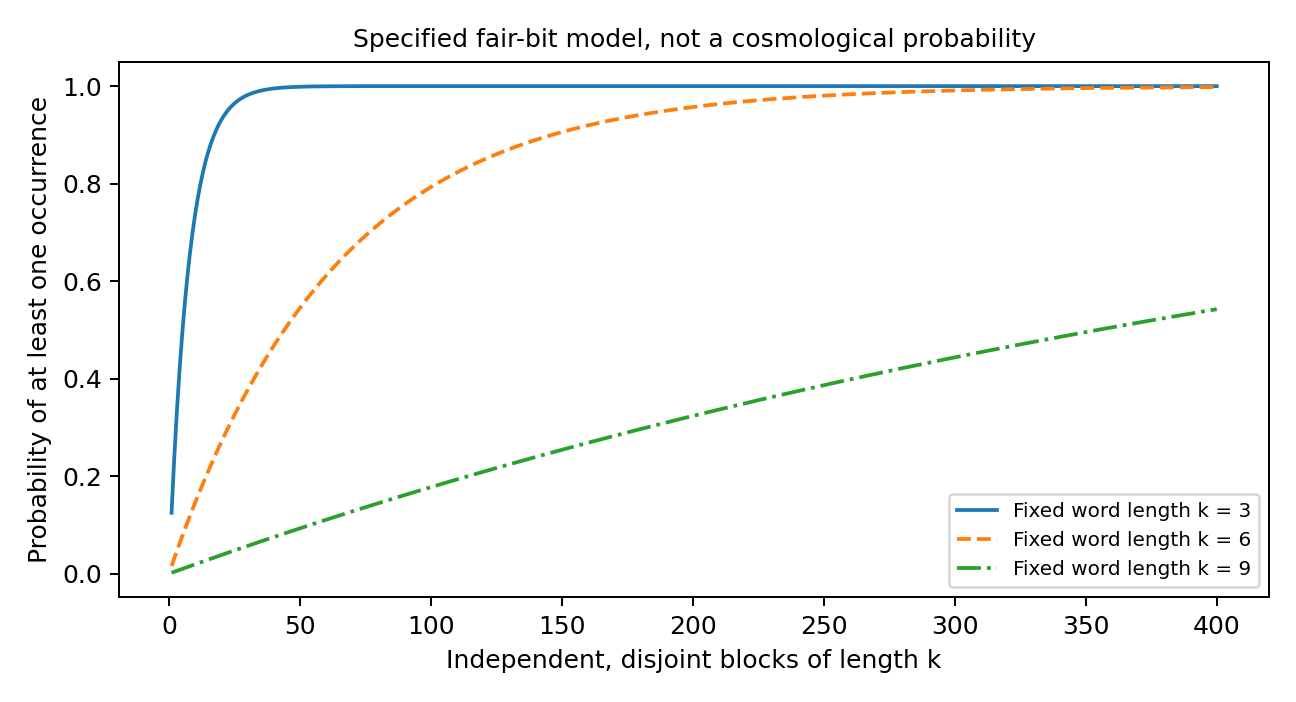
\includegraphics{../../figures/finite_word_probability.png}

\textbf{Figure 1. A conditional probability in the constructed model.
Longer specified words need more independent opportunities to appear.
The curves are not estimates that our universe contains a particular
world, person, heaven or hell.}

\end{minipage}\par\medskip

\subsubsection{5.1.1 Correlated patterns: the stationary-ergodic
extension}\label{correlated-patterns-the-stationary-ergodic-extension}

\textbf{Proposition A1 (standard ergodic corollary).} Let \(\mu\) be a
shift-invariant, ergodic probability measure on
\(\mathcal A^{\mathbb Z}\) for a finite alphabet \(\mathcal A\). For a
finite word \(w\) let \([w]\) be its cylinder at a fixed origin. For
\(\mu\)-almost every sequence, every word with \(\mu([w])>0\) occurs
infinitely often with asymptotic frequency \(\mu([w])\), and no
zero-probability word occurs at any position.

\textbf{Proof.} Apply Birkhoff's pointwise ergodic theorem to the
bounded indicator of each cylinder. Ergodicity makes the invariant
conditional expectation equal to \(\mu([w])\). There are countably many
finite words, so intersect their probability-one convergence events. For
each zero-probability cylinder, stationarity makes its translate at
every integer position have probability zero. The countable union of
those translates and words is null. \(\square\)

This is a direct corollary of a known theorem, not a new probability law
{[}14, Theorem 6.2.1{]}. It extends the independent-bit construction to
many correlated processes. The admissible physical class must be
specified independently; defining admissible to mean positive measure
establishes coverage relative to a measure, not that every physically
possible state has positive measure.

Garriga and Vilenkin's \emph{Many worlds in one} (2001) provides
directly relevant cosmological prior art: under their inflationary and
finite coarse-grained-history premises, they argue for repeated
histories across infinitely many regions {[}15{]}. Their finite-history
argument and the symbolic ergodic theorem are related but not identical.
Infinite regions plus finitely many labels alone guarantees repetition
of some labels, not occurrence of all labels. The realization law and
support must do additional work. The cited cosmological argument does
not make the present physical premises observationally established.

\subsubsection{5.1.2 Ergodicity is sufficient, not
necessary}\label{ergodicity-is-sufficient-not-necessary}

Without ergodicity, Birkhoff still gives a limit
\(\mathbb E[1_{[w]}\mid\mathcal I]\), where \(\mathcal I\) is the
invariant sigma-algebra. In an ergodic decomposition
\(\mu=\int\mu_\xi\,d\lambda(\xi)\) on this standard symbolic space,
typical frequencies are those of the realized component. Every globally
supported finite word occurs in almost every realization precisely when,
for each such word, \(\mu_\xi([w])>0\) for \(\lambda\)-almost every
component. This assertion uses the componentwise ergodic theorem and
countability; it is a coverage criterion, not a claim that the
frequencies equal their mixture averages.

Three examples show the distinctions. A stationary golden-mean Markov
chain forbidding adjacent ones has 13 admissible length-five words, not
all 32. Its ergodic realizations cover those 13 and exclude the other
19. A half-and-half mixture of the all-zero and all-one sequences is
stationary but nonergodic: its length-three support has two words, of
which one realization contains only one. The relevant failure is one of
two supported words, not one of eight supported words. Conversely, a
mixture of independent Bernoulli processes with parameters one quarter
and three quarters is nonergodic but each component has full finite-word
support. Almost every realization still contains every finite binary
word infinitely often, with component-dependent frequencies.
Nonergodicity alone is therefore not an obstruction to finite-pattern
plenitude.

The new finite simulations illustrate the golden-mean support and a
finite sample's coverage. They do not test an infinite almost-sure
theorem by exhaustive observation. Extension to a random field on
\(\mathbb Z^d\) requires a specified measure-preserving shift action and
the appropriate multiparameter averaging theorem; it is not a free
generalization to arbitrary continuous physical worlds.

\subsubsection{5.2 What the construction does not
show}\label{what-the-construction-does-not-show}

The construction supplies its integer index, independent bits and
probability measure. It does not derive geometry, time, energy, a
quantum measurement rule, sentience or a causal process of world
creation. A bit pattern is not automatically an experiencing world. A
physical implementation would need a mapping from the code to lawful
systems, including the resources and subject structure required for
experience.

Every finite word is also much less than every possible infinite world.
There are uncountably many infinite binary configurations, while one
sequence contains only countably many positions at which to begin a
suffix. The finite-word proposition cannot be promoted to realization of
every infinite sequence. Nor does probability one mean that the
exceptional all-zero sequence is logically impossible. The sample-space
semantics remain intact.

A deterministic enumeration can also concatenate every finite word. That
provides another existence construction but places the plenitude
directly in its rule. Neither route makes the realization principle
free. The positive result is coherence under explicit premises; the
actual-world question remains open.

\subsubsection{5.3 A finite-window
comparison}\label{a-finite-window-comparison}

Take a second model: a ring containing L independent fair bits. Compare
it with the infinite independent chain through an experiment that
samples r distinct sites, with r\textless L and without identifying
wraparound or revisiting one physical site under two labels. In both
models every observed r-bit assignment has probability \(2^{-r}\).
Unobserved sites simply marginalize out.

\textbf{Proposition B.} For this specified finite observation design,
the finite-ring and infinite-chain models have identical likelihoods for
every possible outcome.

This does not prove that infinity is forever untestable. It shows that a
particular experiment cannot distinguish these particular models. A
larger domain, repeated-site identification or other structural
assumptions can change their predictions. The lesson is practical:
evidence supports the feature a comparison actually identifies, not the
largest ontology compatible with it.

\subsubsection{5.4 Can this count as a substrate
model?}\label{can-this-count-as-a-substrate-model}

It can be called a minimal generative or configuration model if that
term is defined. One may treat the entire configuration as a single
object with many substructures. That still leaves open whether the
object is physically fundamental or merely a mathematical
representation. The same distribution can be described using many
variables; notation does not settle monism.

The construction is therefore best used as a constructive consistency
test for a restricted AIU component. It shows that certain objections
based solely on infinity or local finiteness are too strong. It does not
supply the empirical bridge for AIU-M, AIU-C or maximal plenitude.

\subsection{6. Infinity, necessity and the
Absolute}\label{infinity-necessity-and-the-absolute}

Cantor's hierarchy and philosophical Absolute should not be collapsed
into one physical magnitude. The fact that a set's power set has larger
cardinality does not show that physical reality instantiates all such
sizes. A physically infinite model can be represented by an ordinary
set. It does not need to be the largest possible mathematical object.
Historical discussions of the Absolute illuminate terminology, not the
truth of a modern cosmology {[}16{]}.

There are several ways to preserve the intended depth without claiming
an invalid theorem. One is unrestricted ontological dependence: every
actual form depends on the same ground. Another is unbounded actual
extent or capacity under a specified physical model. A third is
inexhaustibility of finite descriptions. These may be related in a
developed theory, but none is equivalent by definition to the other two.

A ground that is not located inside effective spacetime need not have
infinite spatial volume in the ordinary sense. Its relevant infinity
might concern histories, relational extent or accessible alternatives
under enlarged domains. It might instead be finite while supporting
emergent spacetime. The empirical implications depend on the exact
representation. Thus the statement that infinity can occur at any point
needs disambiguation: global infinity is not an event that happens at
one coordinate.

Literal unlimited retrievable information in a bounded finite-resource
region encounters distinct physical questions. Entropy bounds have
conditions involving energy, size, entropy definition or light-sheets
{[}17; 18{]}. A maximum bound can constrain an admissible
distinguishable codebook. Finite entropy of a single state alone does
not imply finite support. Neither statement establishes the global size
or experiential nature of the ground.

A proper-class ontology creates additional modelling work but need not
ban all local predictions. A local experiment can have a set-sized
sample space and ordinary observation probabilities even when a
philosophical account refuses a completed set of everything. The
consistency and interpretation of the larger ontology remain separate
problems. Declaring that the totality exceeds formal capture does not
itself yield a prediction.

\subsubsection{6.1 Actual infinity and potentialist
alternatives}\label{actual-infinity-and-potentialist-alternatives}

The author's target includes an actually unbounded reality, not only a
process whose finite descriptions can always be extended. Potentialism
and indefinite extensibility are useful alternatives to examine; Linnebo
and Shapiro (2019) provide a relevant philosophical treatment {[}19{]}.
They must not silently replace the target or be declared mandatory
merely because they ease formal modelling. Actual infinite set models,
extensible-stage models and class-theoretic descriptions can encode
different commitments. Selecting between them requires explicit
philosophical or physical reasons. None is a largest cardinal, and none
proves its own physical realization.

\subsubsection{6.2 Cosmology constrains specified
continuations}\label{cosmology-constrains-specified-continuations}

The DESI DR2 Results IV analysis, version 3, Section VI.4.3, Eq. 36
reports \(10^3\Omega_K=2.1\pm1.1\) for DESI BAO plus Lyman-alpha
full-shape plus CMB, in a curved Lambda-CDM analysis {[}20{]}. This is a
model- and data-combination-dependent curvature constraint, not a direct
measurement of total volume. It does not choose infinity over all finite
alternatives. A compact flat torus illustrates why local flatness alone
is insufficient.

Conversely, failure to settle finiteness against every possible
continuation does not make all finite-versus-infinite comparisons
nondiscriminating. Specified models can predict different topology
signatures, correlation structure or curvature distributions. Their
likelihoods and priors must be stated. The finite-ring theorem concerns
one restricted observation design, not a universal ban on evidence about
global structure. Complete positive-constant-curvature spatial manifolds
can be finite quotients as well as simply connected spheres; simple
connectedness is not required for every finite-volume inference. Other
bearers of unboundedness, including time or generative capacity, remain
distinct.

\subsection{7. Probability without manufactured
precision}\label{probability-without-manufactured-precision}

\subsubsection{7.1 What would an AIU probability
mean?}\label{what-would-an-aiu-probability-mean}

A probability for AIU must be conditional on a hypothesis space,
background information, priors, auxiliary models and an observation
rule. None is supplied by the word infinite. The appropriate comparison
is between sufficiently specified rivals, including their uncertainty
about laws and parameters.

\[
\text{Posterior odds}(H_1:H_0)=\text{Prior odds}(H_1:H_0)\,\frac{\Pr(E\mid H_1)}{\Pr(E\mid H_0)}.
\]

When both rivals exactly reproduce the same observation distribution,
that evidence gives a Bayes factor of one. When either likelihood is
unspecified, no numerical Bayes factor has been earned. It is a mistake
to treat compatibility as probability one, and an equal mistake to treat
lack of a calculated likelihood as probability zero.

The conjunction has its own constraints. Under any common probability
model,

\[
\Pr(H_{\mathrm{AIU}}\mid E)\le\min_{J\in\{M,U,P,C,C^{\text{*}}\}}\Pr(J\mid E),\qquad H_{\mathrm{AIU}}=M\wedge U\wedge P\wedge C\wedge C^{\text{*}}.
\]

Here P inside the event denotes the plenitude proposition; the operator
\(\Pr\) denotes probability. The chain rule expands the conjunction
using conditional probabilities, not an assumed product of five
independent confidence levels. This matters because a person can have a
strong argument for a common basis while having much less evidence for
all possible worlds or one universal subject.

\subsubsection{7.2 A sensitivity illustration, not a
verdict}\label{a-sensitivity-illustration-not-a-verdict}

Suppose, solely for illustration, that a specified model comparison had
Bayes factor ten. A prior probability of 0.01 would become about 0.0917;
a prior of 0.1 would become about 0.5263; a prior of 0.5 would become
about 0.9091. These are arithmetic consequences of the assumptions, not
three estimates of AIU's truth.

\par\medskip\noindent\begin{minipage}{\linewidth}

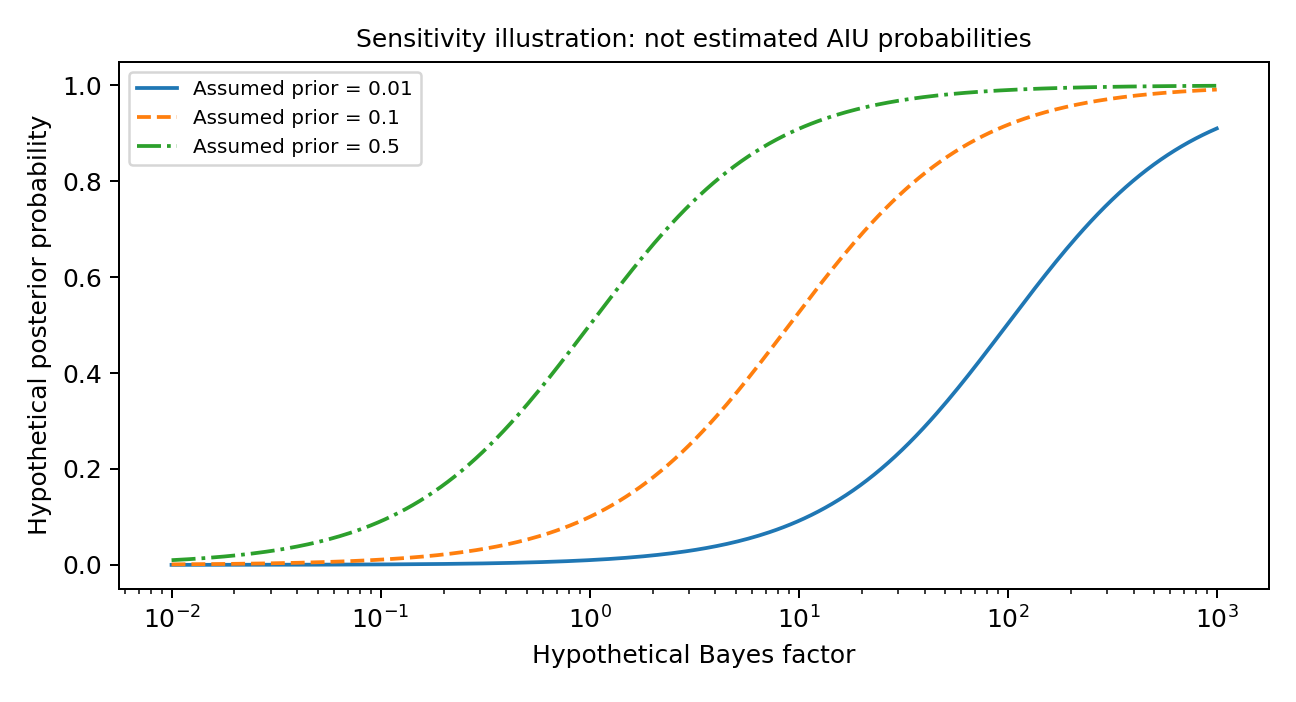
\includegraphics{../../figures/bayes_sensitivity.png}

\textbf{Figure 2. Conditional Bayesian sensitivity. No prior or Bayes
factor on this figure was estimated for AIU. The point is that even a
stated evidence ratio does not uniquely determine a posterior without
the other assumptions.}

\end{minipage}\par\medskip

An explicit non-numerical conclusion can be more rigorous than a precise
invented percentage. One can identify a model as coherent, an argument
as invalid, an empirical claim as constrained, or a comparison as
presently nondiscriminating without pretending to possess a calibrated
probability of ultimate reality.

\subsubsection{7.3 Dependent patterns do not multiply into
certainty}\label{dependent-patterns-do-not-multiply-into-certainty}

For evidence \(E_1,\ldots,E_n\), a valid likelihood factorization is
\(\Pr(E_1\mid H)\Pr(E_2\mid E_1,H)\cdots\). Replacing all conditional
terms with \(\Pr(E_i\mid H)\) assumes conditional independence. Similar
contemplative reports may share biology and traditions; papers may reuse
a dataset; AI systems may reuse text or reasoning; different arguments
may rely on one interpretive premise. Their apparent number can greatly
exceed their independent information.

This does not make convergence worthless. It changes the research
question from how many favourable examples can be listed to how much new
constraint each example supplies. A genuinely surprising out-of-sample
prediction under a well-specified alternative can matter more than
hundreds of repetitions of a familiar description.

\subsection{8. A pattern-and-indicator
ledger}\label{a-pattern-and-indicator-ledger}

Table 4 shows how the programme should treat its principal indicators.
The entries are analytical distinctions, not numerical weights and not a
vote on AIU.

\Needspace{12\baselineskip}

\textbf{Table 4. Indicators, competing explanations and discriminating
work}

\begin{longtable}[]{@{}
  >{\raggedright\arraybackslash}p{(\columnwidth - 6\tabcolsep) * \real{0.2500}}
  >{\raggedright\arraybackslash}p{(\columnwidth - 6\tabcolsep) * \real{0.2500}}
  >{\raggedright\arraybackslash}p{(\columnwidth - 6\tabcolsep) * \real{0.2500}}
  >{\raggedright\arraybackslash}p{(\columnwidth - 6\tabcolsep) * \real{0.2500}}@{}}
\toprule\noalign{}
\begin{minipage}[b]{\linewidth}\raggedright
Indicator
\end{minipage} & \begin{minipage}[b]{\linewidth}\raggedright
Why it motivates AIU
\end{minipage} & \begin{minipage}[b]{\linewidth}\raggedright
Strong alternative explanation
\end{minipage} & \begin{minipage}[b]{\linewidth}\raggedright
Next discriminating task
\end{minipage} \\
\midrule\noalign{}
\endhead
\bottomrule\noalign{}
\endlastfoot
Successful unifications in physics & Common underlying organization can
replace apparent plurality & Shared mathematical representation with
multiple primitives & Compare complete models and independently
recovered phenomena \\
Entangled joint states & The whole has structure not fixed by
independent marginals & Composite quantum systems without substance
monism & State which ontology adds a distinctive prediction or
explanatory constraint \\
Local records in effective physics & Differentiated forms can share
common dynamics & Ordinary decoherence with supplied geometry and
preparation & Test an independently motivated pre-geometric
implementation \\
Boundaryless or near-flat cosmological possibilities & Finite
observational horizons do not bound total reality & Compact finite
geometry or other global continuations & Compare topology and
model-conditioned predictions, not curvature alone \\
Convergent unity reports & Ordinary self-boundaries may not exhaust
experience & Shared cognitive mechanisms and interpretive learning &
Measurement invariance, negative cases and content-specific
reliability \\
Low-structure states yielding organization & A common ground can have
many forms & Supplied laws, perturbations and resource gradients &
Identify exactly which input does the explanatory work \\
Neural dependence of human experience & Could be a constraint on how
local perspectives appear & Physical realization models with explicit
neural mechanisms & Compare subject and intervention predictions, not
generic labels \\
Mathematical infinite constructions & Some forms of unbounded richness
are coherent & Formal existence without physical realization & Supply
physical correspondence and an observation measure \\
\end{longtable}

The ledger avoids two extremes. It does not classify every compatible
pattern as confirmation. It also does not insist that philosophical
explanation can have value only after a laboratory experiment. A
reasoned metaphysical comparison can be substantive, provided its
premises, explanatory criteria and alternatives are made explicit.

\subsection{9. The major rival accounts and their strongest
challenges}\label{the-major-rival-accounts-and-their-strongest-challenges}

These are reconstructed positions, not statements issued by external
scholars in a completed panel. Real advocates may reject some
formulations; that is one reason to seek domain-qualified review rather
than treat the table as a settled debate.

\subsubsection{9.1 Finite common-ground
realism}\label{finite-common-ground-realism}

This rival accepts one ground but denies that unity requires infinity. A
finite quantum or relational model can contain many differentiated
patterns and complex experiences if the relevant realization theory
permits them. Its strongest objection is that AIU has not shown why
adding U explains any particular observation better. The AIU reply must
identify a feature that finite alternatives cannot reproduce, or explain
why an unbounded account is substantially more constrained and
economical. Merely saying a finite ground would need an outside repeats
the boundary error.

\subsubsection{9.2 Plural physical
realism}\label{plural-physical-realism}

This rival treats some plurality of physical components as fundamental
while allowing their states and interactions to be deeply relational. It
need not imagine completely isolated little objects. Its objection is
that a single ground may add a metaphysical label without reducing
physical assumptions. AIU's best reply is to show a genuine dependence
relation or unification that removes otherwise independent postulates. A
global mathematical description alone is insufficient.

\subsubsection{9.3 Structural or process
realism}\label{structural-or-process-realism}

Ontic structural realism gives relational structure explanatory
priority. Process ontology instead emphasizes events or becoming, and
need not reduce to a timeless structure. Both can reject a further
substance behind relations, but they offer different resources for
explaining persistence and change. Both can agree with much of the
substrate research while rejecting the image of one underlying stuff.
Their shared question is what the word substrate contributes beyond the
relational structure. AIU can answer by defining the ground as that
structure, but doing so relinquishes any additional material-goo claim.
A conscious-ground extension would still require its own argument.

\subsubsection{9.4 Neutral and dual-aspect
monism}\label{neutral-and-dual-aspect-monism}

Neutral monism offers a basis not initially classified as either
ordinary mentality or ordinary matter. Dual-aspect monism treats mental
and physical descriptions as irreducible aspects of a common reality.
These positions need not have identical commitments about their ground.
They can make unity plausible while leaving C*'s universal-subject claim
open. Their advantage is avoiding an immediate inference from structural
physics to consciousness. Their challenge is to specify the relation
between the base and its aspects without simply renaming the explanatory
gap. AIU-C must show why experiential fundamentality explains more than
these less committal alternatives.

\subsubsection{9.5 Panpsychist and cosmopsychist
accounts}\label{panpsychist-and-cosmopsychist-accounts}

Panpsychist accounts begin with experiential or proto-experiential
features at a basic level; cosmopsychist accounts begin with a
fundamental whole. The former faces a combination problem, the latter a
differentiation or decomposition problem. Naming one ground does not
decide which grain is a subject. A useful comparison asks how private
viewpoints, split or altered access, and non-biological realizations are
individuated. The existence of these problems does not logically
disprove experiential fundamentals, but it prevents treating them as a
completed explanation {[}10{]}.

\subsubsection{9.6 Idealist and physical-realization
accounts}\label{idealist-and-physical-realization-accounts}

An idealist model takes experience or mentality as fundamental and must
recover the lawfulness of shared observations. A physical-realization
model must explain how the organization of a physical system realizes
experience. Either can be made so flexible that every result is
accommodated. The productive test is between constrained versions: which
systems are subjects, how interventions alter experience, and what
predictions differ before the data are collected? Generic labels are not
complete statistical models.

\subsubsection{9.7 Methodological
empiricism}\label{methodological-empiricism}

This position suspends the ultimate ontological choice while studying
the shared observable structure. Its strongest objection is that many
AIU proposals have no unique empirical consequence. AIU's strongest
reply is that science also depends on conceptual interpretation, and
foundational questions can motivate new models before new predictions
are available. Both points stand. The consequence should be appropriate
classification and targeted development, not either metaphysical
certainty or a prohibition on metaphysical research.

\subsection{10. Consciousness, individuation and the proposed
dream}\label{consciousness-individuation-and-the-proposed-dream}

A literal cosmic-dream account owes more than a metaphor. It must
specify what is experiencing, how differentiated viewpoints arise, why
their access is limited, and how intersubjectively stable observations
emerge. A schematic map e\_j = B\_j(s) from ground state s to
perspective j may organize the question, but the function B\_j contains
the central explanatory burden. Writing it does not explain
phenomenality.

The claim can be separated into experiential character of the ground,
unity of its subjectivity, and the relation between local subjects and
that subject. These need not rise or fall together. A neutral common
ground with local experience is not identical to one cosmic mind. A
common conscious ground with irreducibly private perspectives still
needs a rule for their numerical identity and continuity.

Physical constraints remain relevant where a conscious-ground theory
makes physical commitments. IIT, for example, uses specified causal and
partition conditions rather than a generic measure of unity {[}21{]}. A
conclusion internal to that theory is not a theory-independent disproof
of consciousness beyond its model. Conversely, a claimed cosmic subject
cannot simply ignore causal-model assumptions while invoking IIT as
evidence in its favour.

The paper does not infer that a copy of a person's physical pattern is
the same continuing person. It also does not infer infinite pleasure or
pain from an infinite number of finite episodes. Actual realization,
recurrence, valence magnitude and personal identity are distinct
obligations. Heavens and hells can remain names for proposed
experiential possibilities, but their actual infinite realization is not
established by the word infinity.

\subsubsection{10.1 Affirmative AIU variants, not one ambiguous
claim}\label{affirmative-aiu-variants-not-one-ambiguous-claim}

\Needspace{12\baselineskip}

\textbf{Table 5. Main variants kept active for reasoned comparison}

\begin{longtable}[]{@{}
  >{\raggedright\arraybackslash}p{(\columnwidth - 4\tabcolsep) * \real{0.3333}}
  >{\raggedright\arraybackslash}p{(\columnwidth - 4\tabcolsep) * \real{0.3333}}
  >{\raggedright\arraybackslash}p{(\columnwidth - 4\tabcolsep) * \real{0.3333}}@{}}
\toprule\noalign{}
\begin{minipage}[b]{\linewidth}\raggedright
Variant
\end{minipage} & \begin{minipage}[b]{\linewidth}\raggedright
Positive commitment
\end{minipage} & \begin{minipage}[b]{\linewidth}\raggedright
Distinctive burden
\end{minipage} \\
\midrule\noalign{}
\endhead
\bottomrule\noalign{}
\endlastfoot
AIU-R: relational ground & Every actual entity depends on one generative
relational basis; effective forms need not be primitive & Show a
nontrivial dependence account rather than merely collecting everything
into one set \\
AIU-U: unbounded ground & AIU-R plus no finite bound on a specified
global extent, history depth or distinguishable capacity & Name the
bearer and compare actual finite alternatives; local continuum
mathematics alone is insufficient \\
AIU-C: experiential ground & In the author's nested variant, AIU-U plus
intrinsically experiential reality & Explain the experiential-physical
relation; experiential fundamentality alone does not logically imply
U \\
AIU-C*: cosmic-subject extension & AIU-C plus one unified subject with
genuine local perspectives & Supply phenomenal unity, private access and
individuation rules; common substance does not supply
co-consciousness \\
\end{longtable}

Plenitude is an additional P parameter of any variant, not a hidden
consequence of the letters AIU. P-finite says every finite pattern in a
stated admissible class is realised. P-history says every admissible
complete history is realised. P-modal says every logically coherent
reality is actual. These have different measures, cardinality issues and
observation burdens. The author's preferred strongest vision remains
AIU-C* with a strong P commitment; the weaker variants are comparison
points, not a covert redefinition of that vision.

\subsubsection{10.2 Subject maps and observational
equivalence}\label{subject-maps-and-observational-equivalence}

A candidate model must specify at least a ground-state or history space
S, laws D, an observation kernel O, a subject assignment Sigma(s), and a
mapping B\_j from the relevant ground history to the contents accessible
to perspective j. O is a rule for public experimental outcomes; B\_j is
a proposed experiential bridge, not an equation that solves
consciousness simply by naming it. A cosmic-subject model must explain
why local subjects do not share unrestricted memory or access. A
local-subject model must explain what binds each subject. These are
rival explanatory burdens, not an automatic victory for either account.

There is a precise identification limit. Suppose two complete models,
after integrating over their declared auxiliary parameters, assign the
same probability to every event in a specified observation family. Then
that family gives likelihood ratio one wherever the common probability
is nonzero. No amount of repetition of those same kinds of observations
separates the models. The conclusion is local to that family and model
pair. It does not prove all ontological questions meaningless or every
future observation uninformative.

Conversely, absence of a numerical likelihood is not likelihood ratio
one. An unfinished cosmic-subject proposal may have no specified
prediction at all. The constructive next step is to constrain B\_j or O
enough that an alternative would expect a different outcome, or to argue
a demonstrable reduction in independent explanatory assumptions. A small
p-value in a quantum-record calculation supplies neither bridge by
itself.

\subsubsection{10.2.1 Candidate subject accounts and the objections they
must
answer}\label{candidate-subject-accounts-and-the-objections-they-must-answer}

A subject account may begin with explicit philosophical commitments
rather than a numerical function. Table 6 distinguishes the authors'
proposals and the scope of the source material used, including a
publisher abstract where the full chapter was unavailable. Distinct
proposals must not be collapsed into one supposedly established
solution.

\Needspace{12\baselineskip}

\textbf{Table 6. Primary-source subject accounts and their open burdens}

\begin{longtable}[]{@{}
  >{\raggedright\arraybackslash}p{(\columnwidth - 4\tabcolsep) * \real{0.3333}}
  >{\raggedright\arraybackslash}p{(\columnwidth - 4\tabcolsep) * \real{0.3333}}
  >{\raggedright\arraybackslash}p{(\columnwidth - 4\tabcolsep) * \real{0.3333}}@{}}
\toprule\noalign{}
\begin{minipage}[b]{\linewidth}\raggedright
Approach
\end{minipage} & \begin{minipage}[b]{\linewidth}\raggedright
Claim in the primary source
\end{minipage} & \begin{minipage}[b]{\linewidth}\raggedright
Critical question and checked scope
\end{minipage} \\
\midrule\noalign{}
\endhead
\bottomrule\noalign{}
\endlastfoot
Kastrup, dissociation-based idealism & Living organisms are dissociated
centres within cosmic consciousness; his association-graph analogy
models restricted experiential access & Does lost associative access
suffice for distinct subjects? Sections 8 and 9 propose the account;
Section 12 addresses brain-experience correlations. This is
philosophical extrapolation, not experimental confirmation of cosmic
dissociation {[}22{]} \\
Albahari, perennial idealism & The ground is aperspectival, not an
enlarged perspectival cosmic observer. Dispositional subjects bounded by
imagery account for manifestation & What constrains those dispositions
and their correspondence to observations? Abstract and Sections 3 to 5
inspected. An aperspectival ground is not automatically the one-subject
C* hypothesis {[}23{]} \\
Nagasawa and Wager, priority cosmopsychism & The cosmos is fundamental
and phenomenally propertied; local parts depend on the whole &
Whole-first dependence does not alone individuate private subjects.
Publisher chapter abstract and pages 113-129 verified; full chapter
argument not assessed here {[}24{]} \\
Miller, decombination critique & Structural phenomenal unity and
disunity create a problem distinct from qualitative heterogeneity & His
criticism targets transferring one proposed solution, not every possible
conscious-ground theory. Published article, Sections 2 and 3, inspected;
2021, pages 112-125 {[}25{]} \\
\end{longtable}

Kastrup provides more than a label: his Section 9 proposes associations
among phenomenal contents and dissociation between parts of that
network. Yet ordinary dissociation does not, without another argument,
establish a cosmic implementation. Albahari deliberately avoids treating
the universal ground as another bounded perspective. These are different
ontological commitments, not interchangeable evidence for C*. Both
remain candidates to assess, not validated subject-selection algorithms.

Miller distinguishes qualitative variety within experience from the
unity and boundaries that individuate subjects. This challenges the
automatic transfer of Schaffer's response to heterogeneity into a
solution of decombination. It does not establish that priority monism
itself is true, nor does it rule out every alternative individuation
principle. The priority-monism argument in Section 3.3 therefore remains
motivation for M, not proof of C*.

The next comparative step is to state which subject relations and
observation rules each proposal actually constrains, and distinguish
those from new rules introduced by this programme. A named rival may
assign different probabilities to ordinary intervention or access
outcomes even when both accounts permit them. No clinical intervention
or diagnosis is proposed here, and neural results are not converted into
metaphysical verdicts by analogy alone.

\subsubsection{10.2.2 Worked comparison: a common ground with or without
a cosmic
subject}\label{worked-comparison-a-common-ground-with-or-without-a-cosmic-subject}

Consider a deliberately minimal operational system with two binary
registers A and B. Initially they are independent fair bits. An
intervention sets A to a chosen value a. One later update leaves A
unchanged and, when a communication link is enabled, sets B equal to A
with probability \(1-\eta\), where \(0<\eta<1/2\). When the link is
disabled, B retains its initially independent bit. Reports read the
corresponding registers without additional noise. This is an
identification-limit illustration with equal observable laws imposed by
construction, not a neural model, a fitted theory of consciousness or a
discovery that published subject accounts are observationally
equivalent.

The shared observation rule is therefore
\[\Pr(R_B=a\mid\operatorname{do}(A=a),\mathrm{link}=1)=1-\eta,\]
\[\Pr(R_B=a\mid\operatorname{do}(A=a),\mathrm{link}=0)=1/2.\] At
\(\eta=0.1\), these are 0.9 and 0.5. The same law specifies the entire
joint report distribution. Repeating the experiment, varying a, or
disabling the link cannot discriminate accounts that retain exactly this
law.

\textbf{Cosmic-subject account.} The physical process is a restricted
expression of a common experiential ground. In addition to local
perspectives with contents A and B, the account posits a unified
ground-level subject. Local accessible content is restricted to the
corresponding register and whatever the stated communication rule
supplies. Ground-level co-consciousness is a further postulate; it is
not defined as communication bandwidth.

\textbf{Nearby rival.} The same common ground and operational process
support the same local perspectives, but there is no additional cosmic
subject. The rival can share the proposed physical continuation,
including a separately stipulated unbounded completion. Thus the
comparison holds the infinity and physical-law commitments fixed and
varies the cosmic-subject commitment, rather than confusing several
changes in ontology.

Under these stipulations both accounts agree on every event in the
declared report/intervention family, so the Bayes factor is one wherever
their common event probability is nonzero. Their subject assignments
differ, even though no readout here observes that difference. This is an
exact identification limit for these constructed accounts, not evidence
that actual subject accounts are equivalent in every possible
experiment. Neither account derives phenomenal experience from a bit
label; both still owe an independently defensible experiential bridge.

The strongest objection to the cosmic-subject account is explanatory
surplus: the additional subject has not reduced any operational or
local-subject assumption in this construction. The strongest reply is
that a cosmic unity principle might independently constrain which local
perspectives can exist and thereby reduce the full theory's unexplained
assumptions. That reply becomes an argument only when the constraint is
supplied. The common observation rule cannot by itself favour either
ontology, and counting one fundamental entity as simpler is insufficient
if extra bridge rules are required. A useful discriminator would be an
independently motivated modification that makes the models assign
different probabilities or excludes different subject configurations
before the relevant observations are inspected. This example is the
present paper's schematic comparison, not a formalization claimed by
Kastrup, Albahari, Nagasawa, Wager or Miller.

\subsubsection{10.3 What the preparation results do, and do not, imply
for
formlessness}\label{what-the-preparation-results-do-and-do-not-imply-for-formlessness}

Conditional Haar typicality is a statement about a specified invariant
distribution on finite quantum states. It is not a statement that
reality without a preferred macroscopic form cannot produce form. A
globally covariant ensemble can contain preparation and coupling
resources that are aligned within each individual draw. Conditioning on
those resources matters. Likewise, an energy-constrained ensemble need
not behave like a full-Hilbert-space Haar ensemble.

The stronger scientific descendant of the original image is therefore
not creation from an absence of every constraint. It is generation of
new effective form from a basis lacking that particular effective form,
under explicit relations, history and selection rules. AIU can make this
a positive explanatory ambition. It must then say what is supplied and
show what is recovered, rather than call supplied laws evidence of
unlimited generativity.

\subsection{11. Empirical routes that could
matter}\label{empirical-routes-that-could-matter}

\subsubsection{11.1 Physical structure and
records}\label{physical-structure-and-records}

A physical research route asks whether independently defined locality
and informative records favour compatible subsystem structures. The
mathematical safeguards and finite quantum examples developed in the
separate methods paper \emph{Frame-Aligned Records} do not yet recover
an unknown spacetime metric. Its original source-off pilot has a
negative mean change relative to frozen evolution. A later paired
factorial extension has positive contrasts between Hamiltonian
orientations at fixed injection. These are different counterfactuals,
not a reversal of one result. Neither reconstructs a metric or
establishes a common infinite ground; both concern supplied finite
dynamics and access. A finite propagation bound does not by itself
identify the mechanism behind the scalar readability contrast.

The correspondence burden includes controlled recovery of the target
regime. A few-body decomposition is not enough. Graphs, symmetries,
effective distances, propagation, matter content and measurement rules
must be classified as supplied inputs or recovered outputs. Existing
emergent-spacetime approaches provide concrete problems and examples,
not transferred confirmation of AIU {[}26; 27{]}.

\subsubsection{11.2 Phenomenology and common
structure}\label{phenomenology-and-common-structure}

A useful first question is whether defined experiential dimensions
survive comparison across adequately sampled groups after translation,
expectations and interpretive vocabulary are addressed. A reanalysis can
begin with a known dataset only after its codebook, permissions and
group sizes are inspected. This release did not analyse participant
data. A new study requires ethics review, informed consent and
safeguards for distress; it need not instruct anyone to induce altered
states.

Experiential description should be separated from metaphysical
interpretation. Blind coding of open accounts can complement predeclared
scales, while negative and ambiguous cases remain eligible. Episode
properties, repeatable capacity, enduring trait change and a tradition's
attribution of enlightenment are not one variable. A recovered common
factor establishes a measurement result within its population, not
universal identical experience. Generic AIU and neurocognitive labels do
not by themselves specify the probability of measurement invariance, so
their likelihood ratio cannot simply be assigned a value near one. A
discriminating comparison requires completed observation models; both
models may assign positive probability to an outcome and still be
distinguishable.

\subsubsection{11.3 Content-specific
correspondence}\label{content-specific-correspondence}

For an experience to support a claim about a referent beyond the
experience, there must be a defensible correspondence. Ordinary
perception earns such warrant through prediction, calibration,
cross-checks and action. An AIU interpretation needs an analogous
account appropriate to its content. A feeling of unlimitedness does not
by itself encode infinitely many independently checkable facts.

Unusual information access is not the sole possible test, and no such
ability follows from monism alone. Ordinary evidence about subject
boundaries and intervention effects may be more tractable. A proposed
anomaly would first need rigorous controls and comparison with multiple
explanations; it would not uniquely identify AIU by defeating one
ordinary account.

\subsubsection{11.4 Observation selection and
measure}\label{observation-selection-and-measure}

A plenitude theory must explain why this kind of observation is
expected, not only why it exists somewhere. Observer-weighting
pathologies can make a proposed cosmology epistemically unstable under
stated assumptions {[}28{]}. Their significance is that realization and
observation measures do substantive work. A claim that every possible
world exists still needs an account of why our records are orderly and
reliable.

This task should be approached as model construction, not as a demand
for a universal probability measure before any local science is
permitted. Specific domains and comparisons can be predictive. Their
success does not automatically validate the unrestricted metaphysical
extension.

\subsection{12. Union, compassion and the independence of ethical
protection}\label{union-compassion-and-the-independence-of-ethical-protection}

The author's conception links union with care and the possibility of
flourishing. That can be a coherent ethical orientation without being a
physics theorem. The descriptive fact that two beings share a ground
does not establish a particular duty unless normative premises are
added. Conversely, their protection need not wait for agreement about
ultimate ontology.

Boundaries also have more than one moral role. A boundary can exclude or
harm; it can protect an organism, preserve agency, allow consent and
support cooperation. Fear and greed cannot be reduced to all forms of
separation without a causal account and evidence. The aspiration to
reduce alienation should therefore be distinguished from erasing
functional differentiation.

A strong AIU ethics can say that no being's experience should be
dismissed merely because it is described as an expression of a larger
whole. It must not convert cosmic unity into permission to sacrifice
vulnerable individuals. People who reject AIU remain fully eligible for
protection and participation. This follows from the ethical commitments
being proposed, not from a measurement of the substrate.

Ethical protection should therefore remain robust across the compared
ontologies. A philosophical preference for unity may guide personal
interpretation, but it must not become a prerequisite for rights,
participation or consideration of suffering. Nor should a numerical
ranking be invented when the evidence and normative assumptions do not
identify one.

\subsection{13. What would change the
assessment?}\label{what-would-change-the-assessment}

Table 7 keeps the research vulnerable to evidence without pretending one
experiment can adjudicate the entire conjunction.

\Needspace{12\baselineskip}

\textbf{Table 7. Update rules for the principal commitments}

\begin{longtable}[]{@{}
  >{\raggedright\arraybackslash}p{(\columnwidth - 4\tabcolsep) * \real{0.3333}}
  >{\raggedright\arraybackslash}p{(\columnwidth - 4\tabcolsep) * \real{0.3333}}
  >{\raggedright\arraybackslash}p{(\columnwidth - 4\tabcolsep) * \real{0.3333}}@{}}
\toprule\noalign{}
\begin{minipage}[b]{\linewidth}\raggedright
Claim
\end{minipage} & \begin{minipage}[b]{\linewidth}\raggedright
Confidence could increase through
\end{minipage} & \begin{minipage}[b]{\linewidth}\raggedright
Confidence could decrease through
\end{minipage} \\
\midrule\noalign{}
\endhead
\bottomrule\noalign{}
\endlastfoot
M: one ground & A constrained common-basis model with superior
independent recovery or a stronger grounding argument & A competing
account that explains the same target with fewer arbitrary bridges;
internal inconsistency \\
U: unboundedness & Comparative support for a specified unbounded
continuation against named finite alternatives & Evidence incompatible
with that continuation, such as a relevant compact topology under its
assumptions \\
G: effective emergence & Controlled approximation and successful
predictions of the target regime & Persistent failure in the declared
model class or proof that the target was supplied as input \\
P: realization richness & A realization theorem whose physical premises
are independently supported & Conserved constraints, inaccessible
sectors or a measure contradicting the claimed coverage \\
C: conscious ground & A constrained individuation rule with
discriminating successful predictions or a stronger philosophical
account & Failed predictions, inability to recover observed
dependencies, or uncontrolled ad hoc repairs \\
Phenomenological relevance & Replicated, well-specified convergence and
validated correspondence & Sampling/translation explanations, failed
generalization, or stronger rival predictions \\
\end{longtable}

Evidence against a model is not necessarily evidence against every
member of its broad family. But that fact must not become immunity by
perpetual retreat. After a predeclared class repeatedly fails, the
programme should record that loss, narrow its claim and justify the next
class independently. Calling every successful theory AIU after the fact
would erase the thesis's distinct content.

Likewise, successful mathematical repairs do not move the ontological
posterior by themselves. They improve the instrument used to investigate
one possible mechanism. A correct map is not evidence that the
destination exists; it is what makes a genuine search possible.

\subsection{14. A focused agenda}\label{a-focused-agenda}

Two tasks have the greatest direct relevance. A physical model must
identify its primitives, recover specified observations and compete with
alternatives on a held-out target. A subject account must explain
private perspectives and shared observations, then state either a
genuine empirical discriminator or an explicit philosophical criterion
of preference. The worked comparison in Section 10.2.2 shows how
identical operational predictions leave a precise ontological
disagreement rather than a fictitious probability verdict.

Further development should close one of these obligations with a proof,
counterexample, model comparison or observation. Repetition of
compatible examples is not a substitute. Conceptual criticism remains
useful when it identifies a genuinely different constraint or exposes a
hidden premise; its value is not measured by the number of approving
reviewers.

\subsection{15. Conclusion: the strongest defensible affirmative
position}\label{conclusion-the-strongest-defensible-affirmative-position}

The affirmative AIU position can be stated without false certainty:
differentiated existence may depend on one generative ground; unbounded
and experiential versions are serious possibilities; mathematics can
clarify their consistency and implications; and patterns in physical
organization and experience can motivate focused investigation. The
preferred strong conjunction remains explicit rather than silently
replaced by generic interdependence.

Its current limitation is not that inquiry is prohibited by an old
unsolved problem. It is that the physical, probabilistic and
experiential bridges have not yet been supplied at the strength the full
claim requires. That is a research agenda with identifiable burdens, not
a licence to announce proof or a reason to terminate the investigation.

A successful programme may confirm a constrained AIU account, reject
part of it, or reveal a better structure not captured by the initial
metaphor. Its standard is whether the resulting account explains and
predicts more accurately while carrying fewer unsupported assumptions.
That is how commitment to the possibility of an infinite union can
remain commitment to truth rather than commitment to a predetermined
answer.

\subsection{Declarations}\label{declarations}

This is a philosophical hypothesis assessment, not an empirical
consciousness study. No human-participant data were collected or
reanalysed. Claude and ChatGPT assisted criticism, calculations, source
retrieval, drafting and production; no AI system is an author, and their
agreement is not independent evidence. The author retains responsibility
for the arguments and final approval. Funding, competing interests and
final correspondence metadata require author confirmation before
submission. Related quantum calculations belong to the separate methods
paper and supplement, not independent confirmations of this ontology.

\subsection{References}\label{references}

{[}1{]} Spinoza, B. (1677). Ethics, Part I, Definition 6 and
Propositions 14, 15 and 33. R. H. M. Elwes translation.
\url{https://www.gutenberg.org/files/3800/3800-h/3800-h.htm}

{[}2{]} Lovejoy, A. O. (1936). The Great Chain of Being: A Study of the
History of an Idea. Harvard University Press. Modern reprint publisher
record:
\url{https://www.routledge.com/The-Great-Chain-of-Being-A-Study-of-the-History-of-an-Idea/Lovejoy/p/book/9781412810265}

{[}3{]} Lewis, D. (1986). On the Plurality of Worlds. Blackwell.
Publisher reprint description:
\url{https://www.wiley-vch.de/en/areas-interest/humanities-social-sciences/on-the-plurality-of-worlds-978-0-631-22426-6}

{[}4{]} Nozick, R. (1981). Philosophical Explanations. Harvard
University Press. Bibliographic lead only in this edition; the relevant
original chapter was not retrieved.

{[}5{]} Tegmark, M. (2008). The Mathematical Universe. Foundations of
Physics 38, 101-150. \url{https://doi.org/10.1007/s10701-007-9186-9} ;
arXiv:0704.0646.

{[}6{]} Shani, I. (2015). Cosmopsychism: A Holistic Approach to the
Metaphysics of Experience. Philosophical Papers 44(3), 389-437.
\url{https://doi.org/10.1080/05568641.2015.1106709}

{[}7{]} Goff, P. (2017). A Conscious Universe. In Consciousness and
Fundamental Reality, Chapter 9, 220-255. Oxford University Press.
\url{https://doi.org/10.1093/oso/9780190677015.003.0009}

{[}8{]} Schaffer, J. (2010). Monism: The priority of the whole. The
Philosophical Review, 119(1), 31-76.
\url{https://www.jonathanschaffer.org/monism.pdf}

{[}9{]} Horodecki, R., et al.~(2009). Quantum entanglement. Reviews of
Modern Physics, 81, 865-942.
\url{https://arxiv.org/abs/quant-ph/0702225}

{[}10{]} Chalmers, D. J. (2016). The combination problem for
panpsychism. In Panpsychism: Contemporary Perspectives, pp.~179-214.
Oxford University Press. \url{https://consc.net/papers/combination.pdf}

{[}11{]} Gamma, A., \& Metzinger, T. (2021). The Minimal Phenomenal
Experience questionnaire. PLOS ONE, 16(7), e0253694.
\url{https://journals.plos.org/plosone/article?id=10.1371/journal.pone.0253694}

{[}12{]} Lindahl, J. R., et al.~(2017). The varieties of contemplative
experience. PLOS ONE, 12(5), e0176239.
\url{https://journals.plos.org/plosone/article?id=10.1371/journal.pone.0176239}

{[}13{]} Springel, V., et al.~(2005). Simulations of the formation,
evolution and clustering of galaxies and quasars. Nature, 435, 629-636.
\url{https://arxiv.org/abs/astro-ph/0504097}

{[}14{]} Durrett, R. (2019). Probability: Theory and Examples, 5th
ed.~Cambridge University Press.
\url{https://sites.math.duke.edu/~rtd/PTE/PTE5_011119.pdf}

{[}15{]} Garriga, J., and Vilenkin, A. (2001). Many worlds in one.
Physical Review D 64, 043511.
\url{https://arxiv.org/html/gr-qc/0102010v2}

{[}16{]} Welch, P., \& Horsten, L. (2016). Reflecting on absolute
infinity. The Journal of Philosophy, 113(2), 89-111.
\url{https://research-information.bris.ac.uk/ws/portalfiles/portal/56264140/AbsInfFIN_revised_October_2015.pdf}

{[}17{]} Bousso, R. (2002). The holographic principle. Reviews of Modern
Physics, 74, 825-874. \url{https://arxiv.org/abs/hep-th/0203101}

{[}18{]} Casini, H. (2008). Relative entropy and the Bekenstein bound.
Classical and Quantum Gravity, 25, 205021.
\url{https://arxiv.org/abs/0804.2182}

{[}19{]} Linnebo, O., and Shapiro, S. (2019). Actual and Potential
Infinity. Nous 53(1), 160-191. \url{https://doi.org/10.1111/nous.12208}

{[}20{]} DESI Collaboration (2026). DESI DR2 Results IV:
Alcock-Paczynski Measurements from the Lyman Alpha Forest and
Cosmological Constraints. arXiv:2607.27410v3, Section VI.4.3, Eq. 36.
\url{https://arxiv.org/html/2607.27410v3}

{[}21{]} Albantakis, L., et al.~(2023). Integrated information theory
(IIT) 4.0. PLOS Computational Biology, 19(10), e1011465.
\url{https://journals.plos.org/ploscompbiol/article?id=10.1371/journal.pcbi.1011465}

{[}22{]} Kastrup, B. (2018). The Universe in Consciousness. Journal of
Consciousness Studies 25(5-6), 125-155.
\url{https://www.imprint.co.uk/wp-content/uploads/2019/03/Kastrup_Open_Access.pdf}

{[}23{]} Albahari, M. (2019). Perennial Idealism: A Mystical Solution to
the Mind-Body Problem. Philosophers' Imprint 19(44), 1-37.
\url{https://quod.lib.umich.edu/p/phimp/3521354.0019.044/1}

{[}24{]} Nagasawa, Y., and Wager, K. (2016). Panpsychism and Priority
Cosmopsychism. In G. Bruntrup and L. Jaskolla (eds.), Panpsychism:
Contemporary Perspectives, 113-129. Oxford University Press.
\url{https://doi.org/10.1093/acprof:oso/9780199359943.003.0005}

{[}25{]} Miller, G. (2021). The Decombination Problem for Cosmopsychism
is not the Heterogeneity Problem for Priority Monism. Journal of
Consciousness Studies 28(3-4), 112-125.
\url{https://philpapers.org/archive/MILTDP-5.pdf}

{[}26{]} Surya, S. (2019). The causal set approach to quantum gravity.
Living Reviews in Relativity, 22, 5.
\url{https://arxiv.org/abs/1903.11544}

{[}27{]} Van Raamsdonk, M. (2010). Building up spacetime with quantum
entanglement. General Relativity and Gravitation, 42, 2323-2329.
\url{https://arxiv.org/abs/1005.3035}

{[}28{]} Carroll, S. M. (2017). Why Boltzmann brains are bad.
arXiv:1702.00850. \url{https://arxiv.org/abs/1702.00850}

\end{document}
